\section{Classification of states}
\begin{definition}[]
    We say that state $j$ is \textit{accessible} from state $i$, written as $ i \to j $, If  $ p^{n}_{ij}>0 $ for some $ n\in\mathds{N} $.\\ 
    We assume every state is accessible from itself since,
    \[
        p^{0}_{ii} = \mathbf{P}(X_{0}=i|X_{0}=i) = 1.
    \]
\end{definition}

\begin{definition}[]
    Two states $i$ and $j$ are said to \textit{communicate} , written as $ i \longleftrightarrow j $, if they are accessible from each other.\\ 
    i.e.
    \[
        i\longleftrightarrow j \implies i \to j \ \And j\to i
    \]
\end{definition}

Communication is an equivalence relation. That means that,
\begin{enumerate}
    \item $ i\longleftrightarrow i $.
    \item if $ i\longleftrightarrow j $ then  $ j\longleftrightarrow i$.
    \item if  $ i\longleftrightarrow j $ and  $ j\longleftrightarrow k $ then  $ i\longleftrightarrow k $.
\end{enumerate}

First two property is obvious for last one, let for some n, m in $ \mathds{N} $ then, $ p^{n}_{ij},p^{m}_{jk}>0 $ by assumption.
By Chapman-Kolmogorov equatation.
\[
    p^{n+m}_{ik} = \sum_{r=0}^{\infty} p^{n}_{ir}p^{m}_{rk} \ge p^{n}_{ij}p^{m}_{jk}>0.
\]
Hence state k is accessible from state i. By same we can see tha converse.

Therefore, the states of a Markov chain can be partitioned into communicating classes such that 
only members of the same class communicate with each other. 
i.e. two states $ i \ \&\ j $ belong to same class if and only if $ i\longleftrightarrow j $.

\begin{example}[]
    Consider the markov chain define in the picture \cref{example of communication}.
\begin{figure}[h]
    \centering
    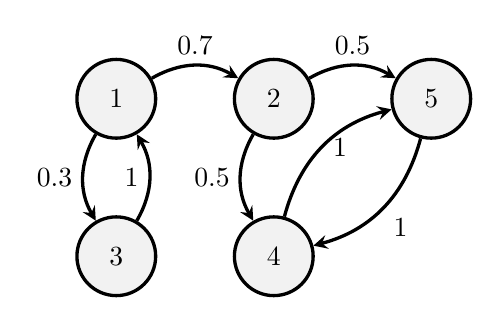
\begin{tikzpicture}[->, >=stealth, auto, very thick, node distance = 2cm, state/.style={circle, draw=black, fill=black!5, very thick, minimum size = 10mm}]
        \node[state] (1) {$1$};
        \node[state] (2) [right of=1] {$2$};
        \node[state] (3) [below of=1] {$3$};
        \node[state] (4) [below of=2] {$4$};
        \node[state] (5) [right of=2] {$5$};

        \path (1) edge [bend right] node [left] {0.3} (3)
              (1) edge [bend left] node [above] {0.7} (2)
              (3) edge [bend right] node {1} (1)
              (2) edge [bend right] node [left] {0.5} (4)
              (2) edge [bend left] node {0.5} (5)
              (4) edge [bend left] node [right] {1} (5)
              (5) edge [bend left] node {1} (4);
    \end{tikzpicture}
    \caption{}
    \label{example of communication}
\end{figure}

Here the classes are $\{ 1,3 \}, \{2\}, \{4,5\}$
\end{example}

\begin{definition}[Irreducible Markov chain]
    A Markov chain is said to be irreducible if it has only one communicating class. That is, every state communicate with each other.\\ 
    That is, for any states $i$, $j$ there is some positive integer $n$ such that the $(i, j)$ entry of $ P^{n} $ is positive.
\end{definition}

A Markov chain that is not irreducible called reducible.

For any state $ i $ and $ j $ define $ f^{n}_{ij} $ to be the probability that, starting from $ i $, the first transition into $ j  $
occurs at $ n $ time. \\ 
i.e. 
\[
    f^{n}_{ij} = \mathbf{P}(X_{n},X_{k}\neq j, k=1,2,\ldots n-1|X_{0}=i).
\]
Let,
\[
    f_{ij}=\sum_{n=0}^{\infty} f^{n}_{ij}
\]

Then, $ f_{ii} $ denote the probability of ever making a transition into step $ j $ when start from state $ i $. 
If $ j $ is not accessible from $ i $ $ f_{ij} $ will be zero.

\begin{definition}[Recurrent and Transient state]
    A state $ j $ of a Markov chain is said to be \textit{recurrent}  $ f_{ii}=1 $ and \textit{transient}  if $ f_{ii}<0 $.
\end{definition}

In other word, if a markov chain start in a recurrent state, there is a guarantee that it will visit that state again in the future
(eventually return to that state with probability 1).
Recurrent states are often considered "absorbing" because once you enter them, you stay there indefinitely.

In contrast, a transient state in a Markov chain is a state where, once you reach it, 
there is a positive probability that you will never return to that state.
i.e. if you begin in a transient state, there's a chance you won't return there.

\begin{proposition}
     In an irreducible Markov chain with a finite state space, all states are recurrent.
\end{proposition}

